\documentclass[a4paper]{article}

%%%%%%%%%%%%%%%%
%%% PREAMBLE %%%
%%%%%%%%%%%%%%%%

%%% PACKAGES %%%
\usepackage{fontspec}                     % set fonts
	\setmainfont{Junicode}
\usepackage[a4paper,margin=3cm]{geometry} % page layout
\usepackage[svgnames]{xcolor}             % rainbowssss *_*
\usepackage{hyperref}                     % enhanced references (links)
	\hypersetup{%
		colorlinks=true,
		allcolors=NavyBlue}
\usepackage{fancyhdr}                     % headers & footers
\usepackage{titling}                      % macros \thetitle, \theauthor
\usepackage{graphicx}                     % enhanced graphics support
	\graphicspath{{img/}}
\usepackage[toc]{glossaries}              % glossaries (obv)
	\setglossarystyle{altlisthypergroup}
	\makeglossaries
	\newglossaryentry{turnstile}
{%
	name=turnstile,
	description={An ingress control device to help with the organizization
	of the passengers’ boarding. Basically a lockable revolving gate with
	three arms. When signalled, the gate unlocks and a single passenger may
	go through by turning one of the arms. After a single rotation, the gate
	locks again, waiting for the next signal.}
}

\newglossaryentry{authentication}
{%
	name=authentication,
	description={The process of verifying the \textit{identity} of the
	passengers.}
}

\newglossaryentry{authorization}
{%
	name=authorization,
	description={The process of veryfying whether an identified passenger
	has \textit{permission} to do something (eg board the bus).}
}

\newglossaryentry{alarm}
{%
	name=alarm,
	description={A device installed at every door that emits light and sound
	to draw attention to certain events. For instance, it signals the end of
	the boarding phase and also turns on in the event of an unauthorized
	boarding attempt.}
}

\newglossaryentry{RFIDScanner}
{%
	name={RFID scanner},
	description={An instrument capable of reading radio frequency
	identification tags. This can be used to effectively identify
	passengers.}
}

\newglossaryentry{boardingController}
{%
	name={boarding controller},
	description={A device responsible for the orchestration of the whole
	boarding phase (signalling doors to open or close, activating the alarm,
	etc).}
}

\usepackage{enumitem}                     % enhanced enumerations
\usepackage{tabularx}                     % enhanced tables
\usepackage{float}                        % 'H' figure placement
\usepackage{rotating}                     % sidewaysfigure
\usepackage[noabbrev]{cleveref}           % clever references
\usepackage{booktabs}                     % pretty tables
\usepackage{tikz}                         % drawings
	\usetikzlibrary{shapes}
\usepackage{subcaption}                   % side-by-side figures & subfigures

%%% OTHER %%%
\setlength\headheight{22.3725pt}

%%% META %%%
\title{Assignment \#3 \\ Behavioural Modelling}
\author{Levendula}
\date{\today}

%%% ADDITIONAL PACKAGE CONFIG %%%
% fancyhdr
\pagestyle{fancy}
\fancyhf{}
\lhead{\theauthor}
\rhead{\thetitle}
\lfoot{\today}
\rfoot{\thepage}

%%%%%%%%%%%%%%%%%%%%%%%%%%%%%%%%%%%%%%%%%%%%%%%%%%%%%%%%%%%%%%%%%%%%%%%%%%%%%%%%

%%%%%%%%%%%%
%%% BODY %%%
%%%%%%%%%%%%

\begin{document}

\begin{titlepage}
	\begin{center}
		
\includegraphics[width=8cm]{logo.jpg}

		\vspace{.2cm}

		\textbf{Budapest University of Technology and Economics} \\
		Faculty of Electrical Engineering and Informatics \\
		Department of Measurement and Information Systems \\

		\vspace{2cm}

		{\huge IT System Design (\texttt{VIMIAC01})}

		\vspace{2cm}

		{\huge \bfseries \thetitle}

		\vspace{.5cm}

		{\Large \theauthor}

		\vspace{.5cm}

		{\Large \today}
	\end{center}

	\vfill{}

	{\large Team members:}

	\vspace{.25cm}

	\begin{tabular}{lll}
		Annamária Gálik &
			\texttt{WGMUO2} &
			ancsi666@gmail.com \\
		Borbála Szilágyi &
			\texttt{COVQ1M} &
			szilagyiborbala8@gmail.com \\
		Bertalan Z. Péter &
			\texttt{QO7CU6} &
			bertalan.peter+uni@bertalanp99.eu
	\end{tabular}

	\vspace{2cm}
\end{titlepage}


\tableofcontents
\listoffigures
\clearpage



% ------------------------------------------------------------------------------
\section{Our task}

We were assigned to model the behaviour of some components related to boarding
using state machine and activity diagrams.

First, we modelled the operation of the bus's doors by means of a state machine
diagram. The behaviour of the doors was already defined in some specific cases
on sequence diagrams, which we made sure to conform to.

In the second task, we created an activity diagram describing the
\gls{RFIDScanner} based on the textual user manual.

As a final task, we made another state machine diagram which models the
behaviour of the \gls{boardingController} based on the other components'
behaviour—diagrams for some components have been given to us, such as the
\gls{turnstile}'s state machine diagram. We made sure to adhere to the critical
requirements.


% ------------------------------------------------------------------------------
\section{Solutions}


% - - - - - - - - - - - - - - - - - - - - - - - - - - - - - - - - - - - - - - -
\subsection{The state machine representation of the door's behaviour}

The door intutively has two states: \texttt{Opened} and \texttt{Closed}.

Successfully transitioning into the \texttt{Opened} and \texttt{Closed} states
results in respective \texttt{Opened} and \texttt{Closed} signals being sent.

When transitioning out of the \texttt{Opened} state, it is possible that the
door cannot close properly due to being blocked: in this case, a
\texttt{Blocked} signal is emitted and the door continues being \texttt{Opened}.

See \cref{fig:stm-DoorBehavior} for the state machine diagram. All the actions
seen on the transitions can be seen on \cref{fig:stm-DoorBehavior-actions}.

All the activities seen on the transitions can be seen on
\cref{fig:stm-DoorBehavior-effects}.

\begin{figure}[p]
	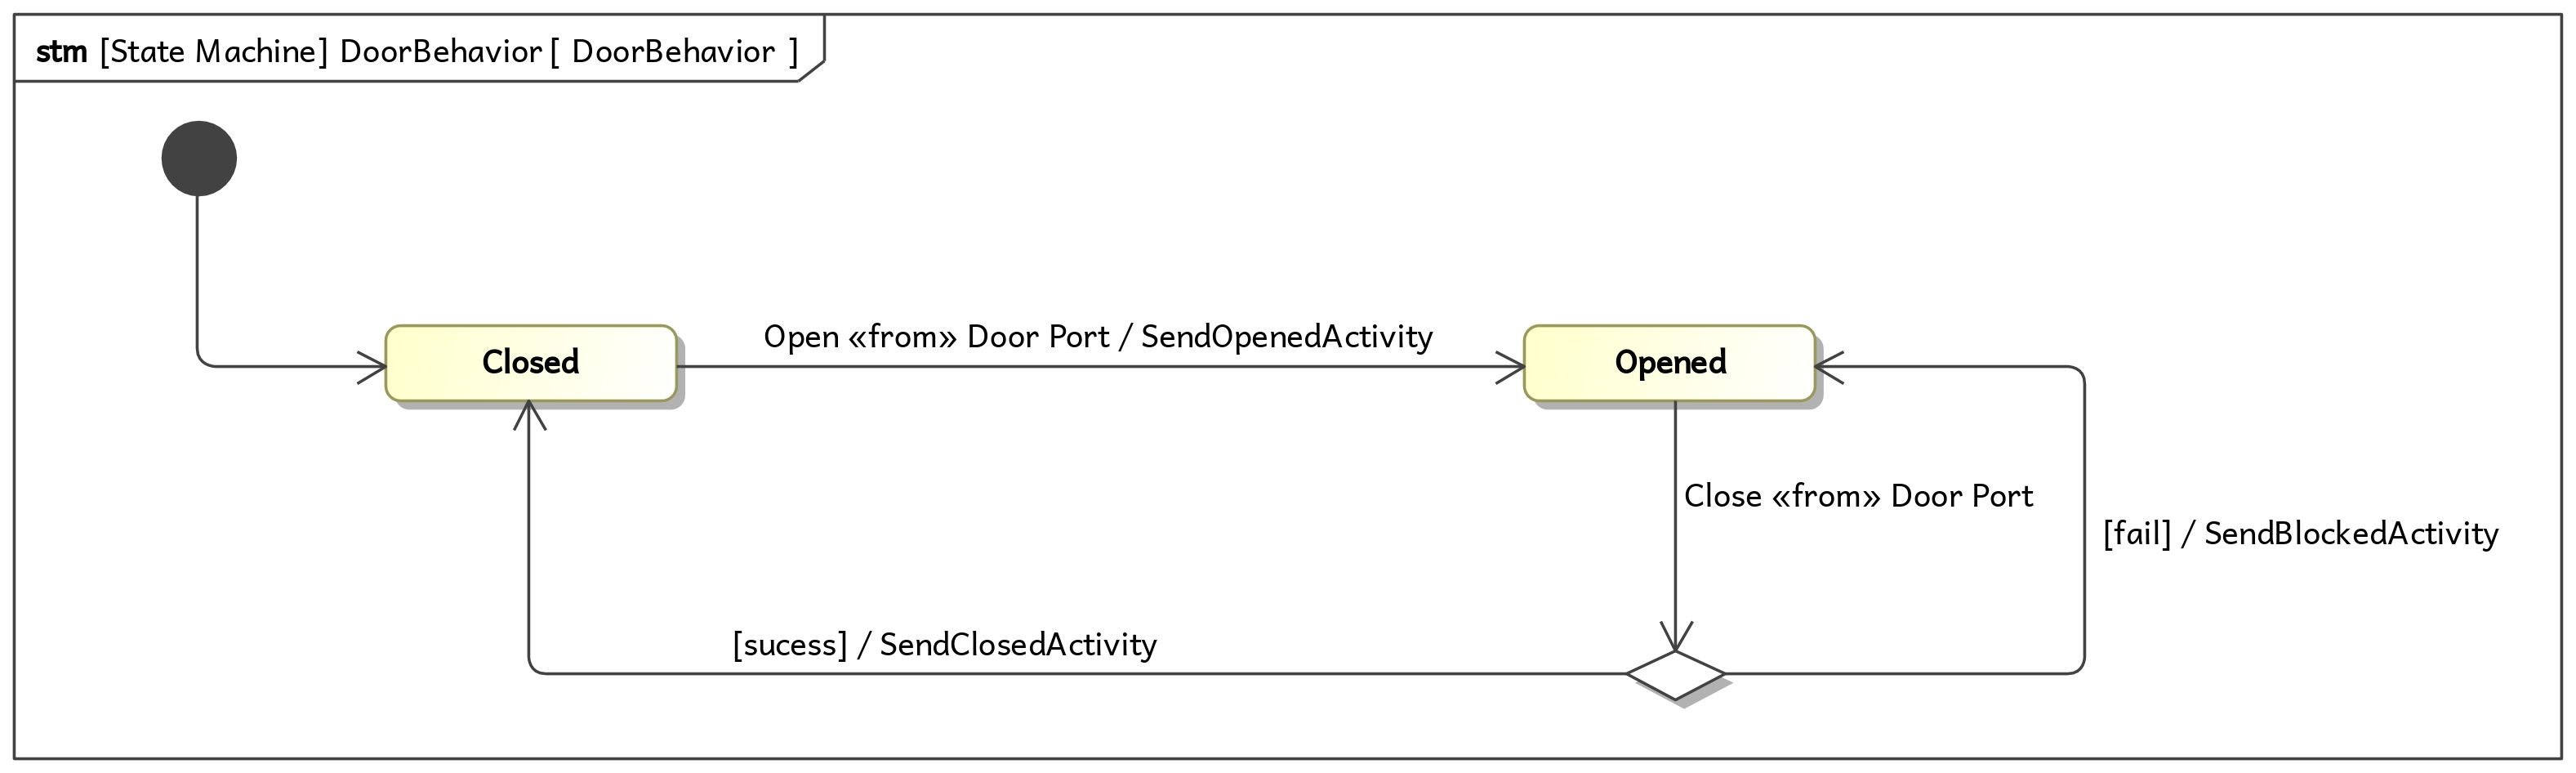
\includegraphics[width=\textwidth]{stm-DoorBehavior.jpg}
	\caption{State machine diagram modelling the door's behaviour}%
	\label{fig:stm-DoorBehavior}
\end{figure}

\begin{figure}
	\begin{subfigure}{.33\textwidth}
		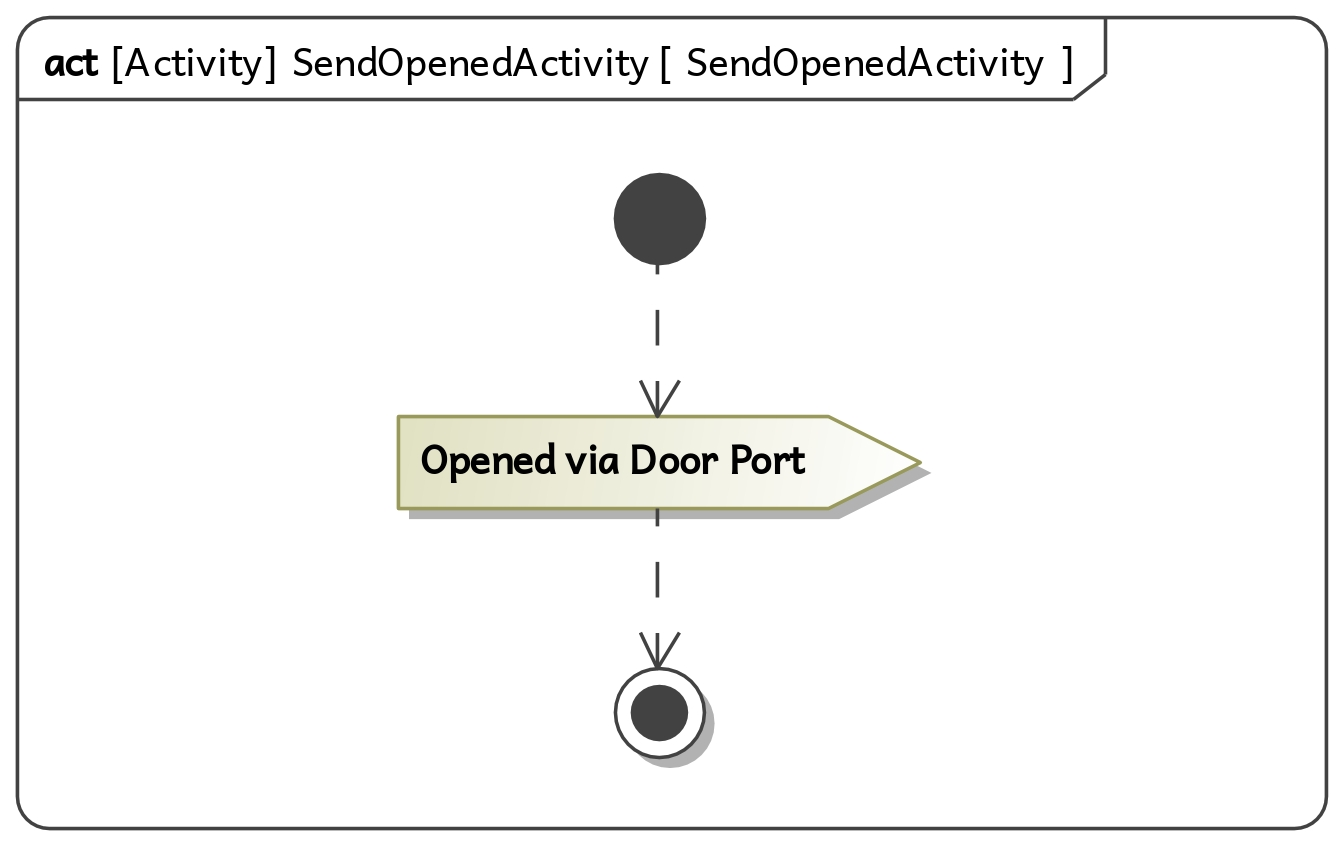
\includegraphics[width=\textwidth]
		{stm-DoorBehavior-SendOpenedActivity.jpg}
	\end{subfigure}
	\begin{subfigure}{.33\textwidth}
		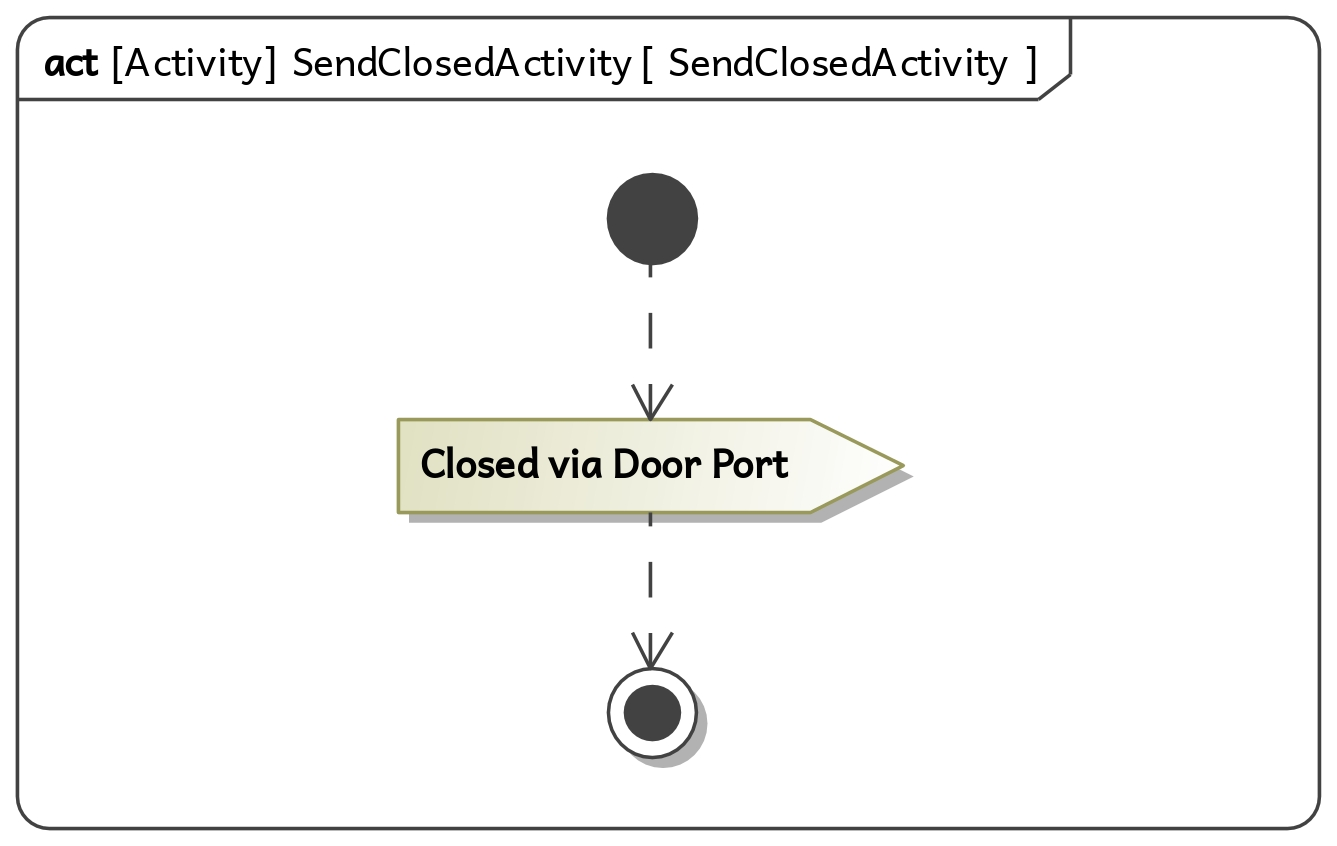
\includegraphics[width=\textwidth]
		{stm-DoorBehavior-SendClosedActivity.jpg}
	\end{subfigure}
	\begin{subfigure}{.33\textwidth}
		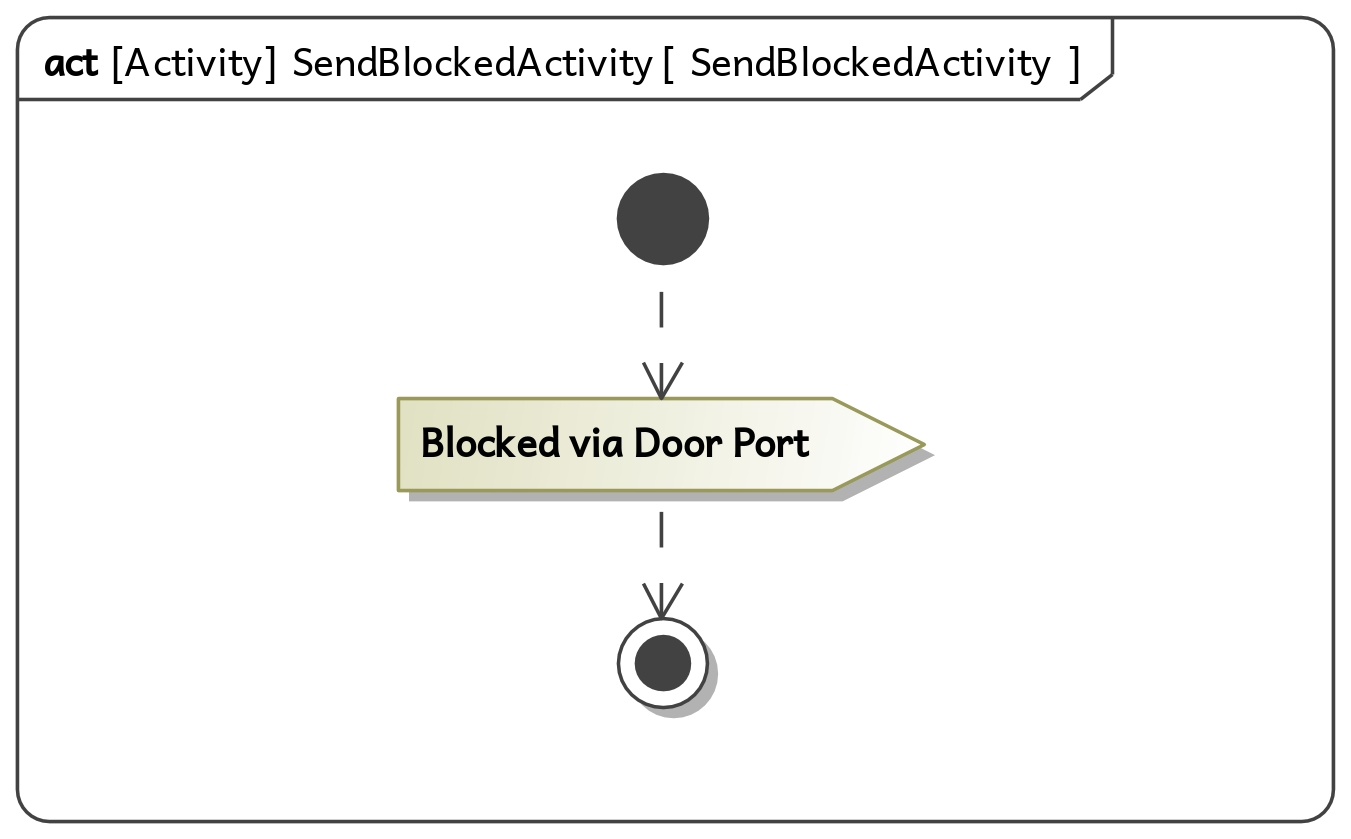
\includegraphics[width=\textwidth]
		{stm-DoorBehavior-SendBlockedActivity.jpg}
	\end{subfigure}
	\caption{Activity diagrams for the transition actions seen on
		\cref{fig:stm-DoorBehavior}}%
	\label{fig:stm-DoorBehavior-actions}
\end{figure}


% - - - - - - - - - - - - - - - - - - - - - - - - - - - - - - - - - - - - - - -
\subsection{Activity diagram for the RFID scanner}

As described in the \gls{RFIDScanner}'s user manual, the scanner initially
listens for a \texttt{Start} signal on its port. Upon receiving the signal, the
scanning process begins.

The process may end in three ways:

\begin{enumerate}[label=\Alph*)]
	\item The RFID raw data is read and processed within five seconds. In
		this case, the results are given to the \gls{boardingController}
		in a \texttt{SuccessfulScan} signal.

	\item Reading and processing of the data cannot be completed within the
		five second window. A \texttt{Timeout} signal is sent.

	\item The scanner receives a \texttt{Stop} signal.
\end{enumerate}

In all three cases, the scanning process terminates and the scanner resumes
listening for the \texttt{Start} signal.

We have modelled this behaviour by enclosing the scanning process in an
\emph{interruptible region} and specifying the flows leaving the ending actions
that correspond to the possible cases as \emph{interrupting}.

The activity diagram can be found on \cref{fig:act-ScannerBehavior}.

\begin{figure}
	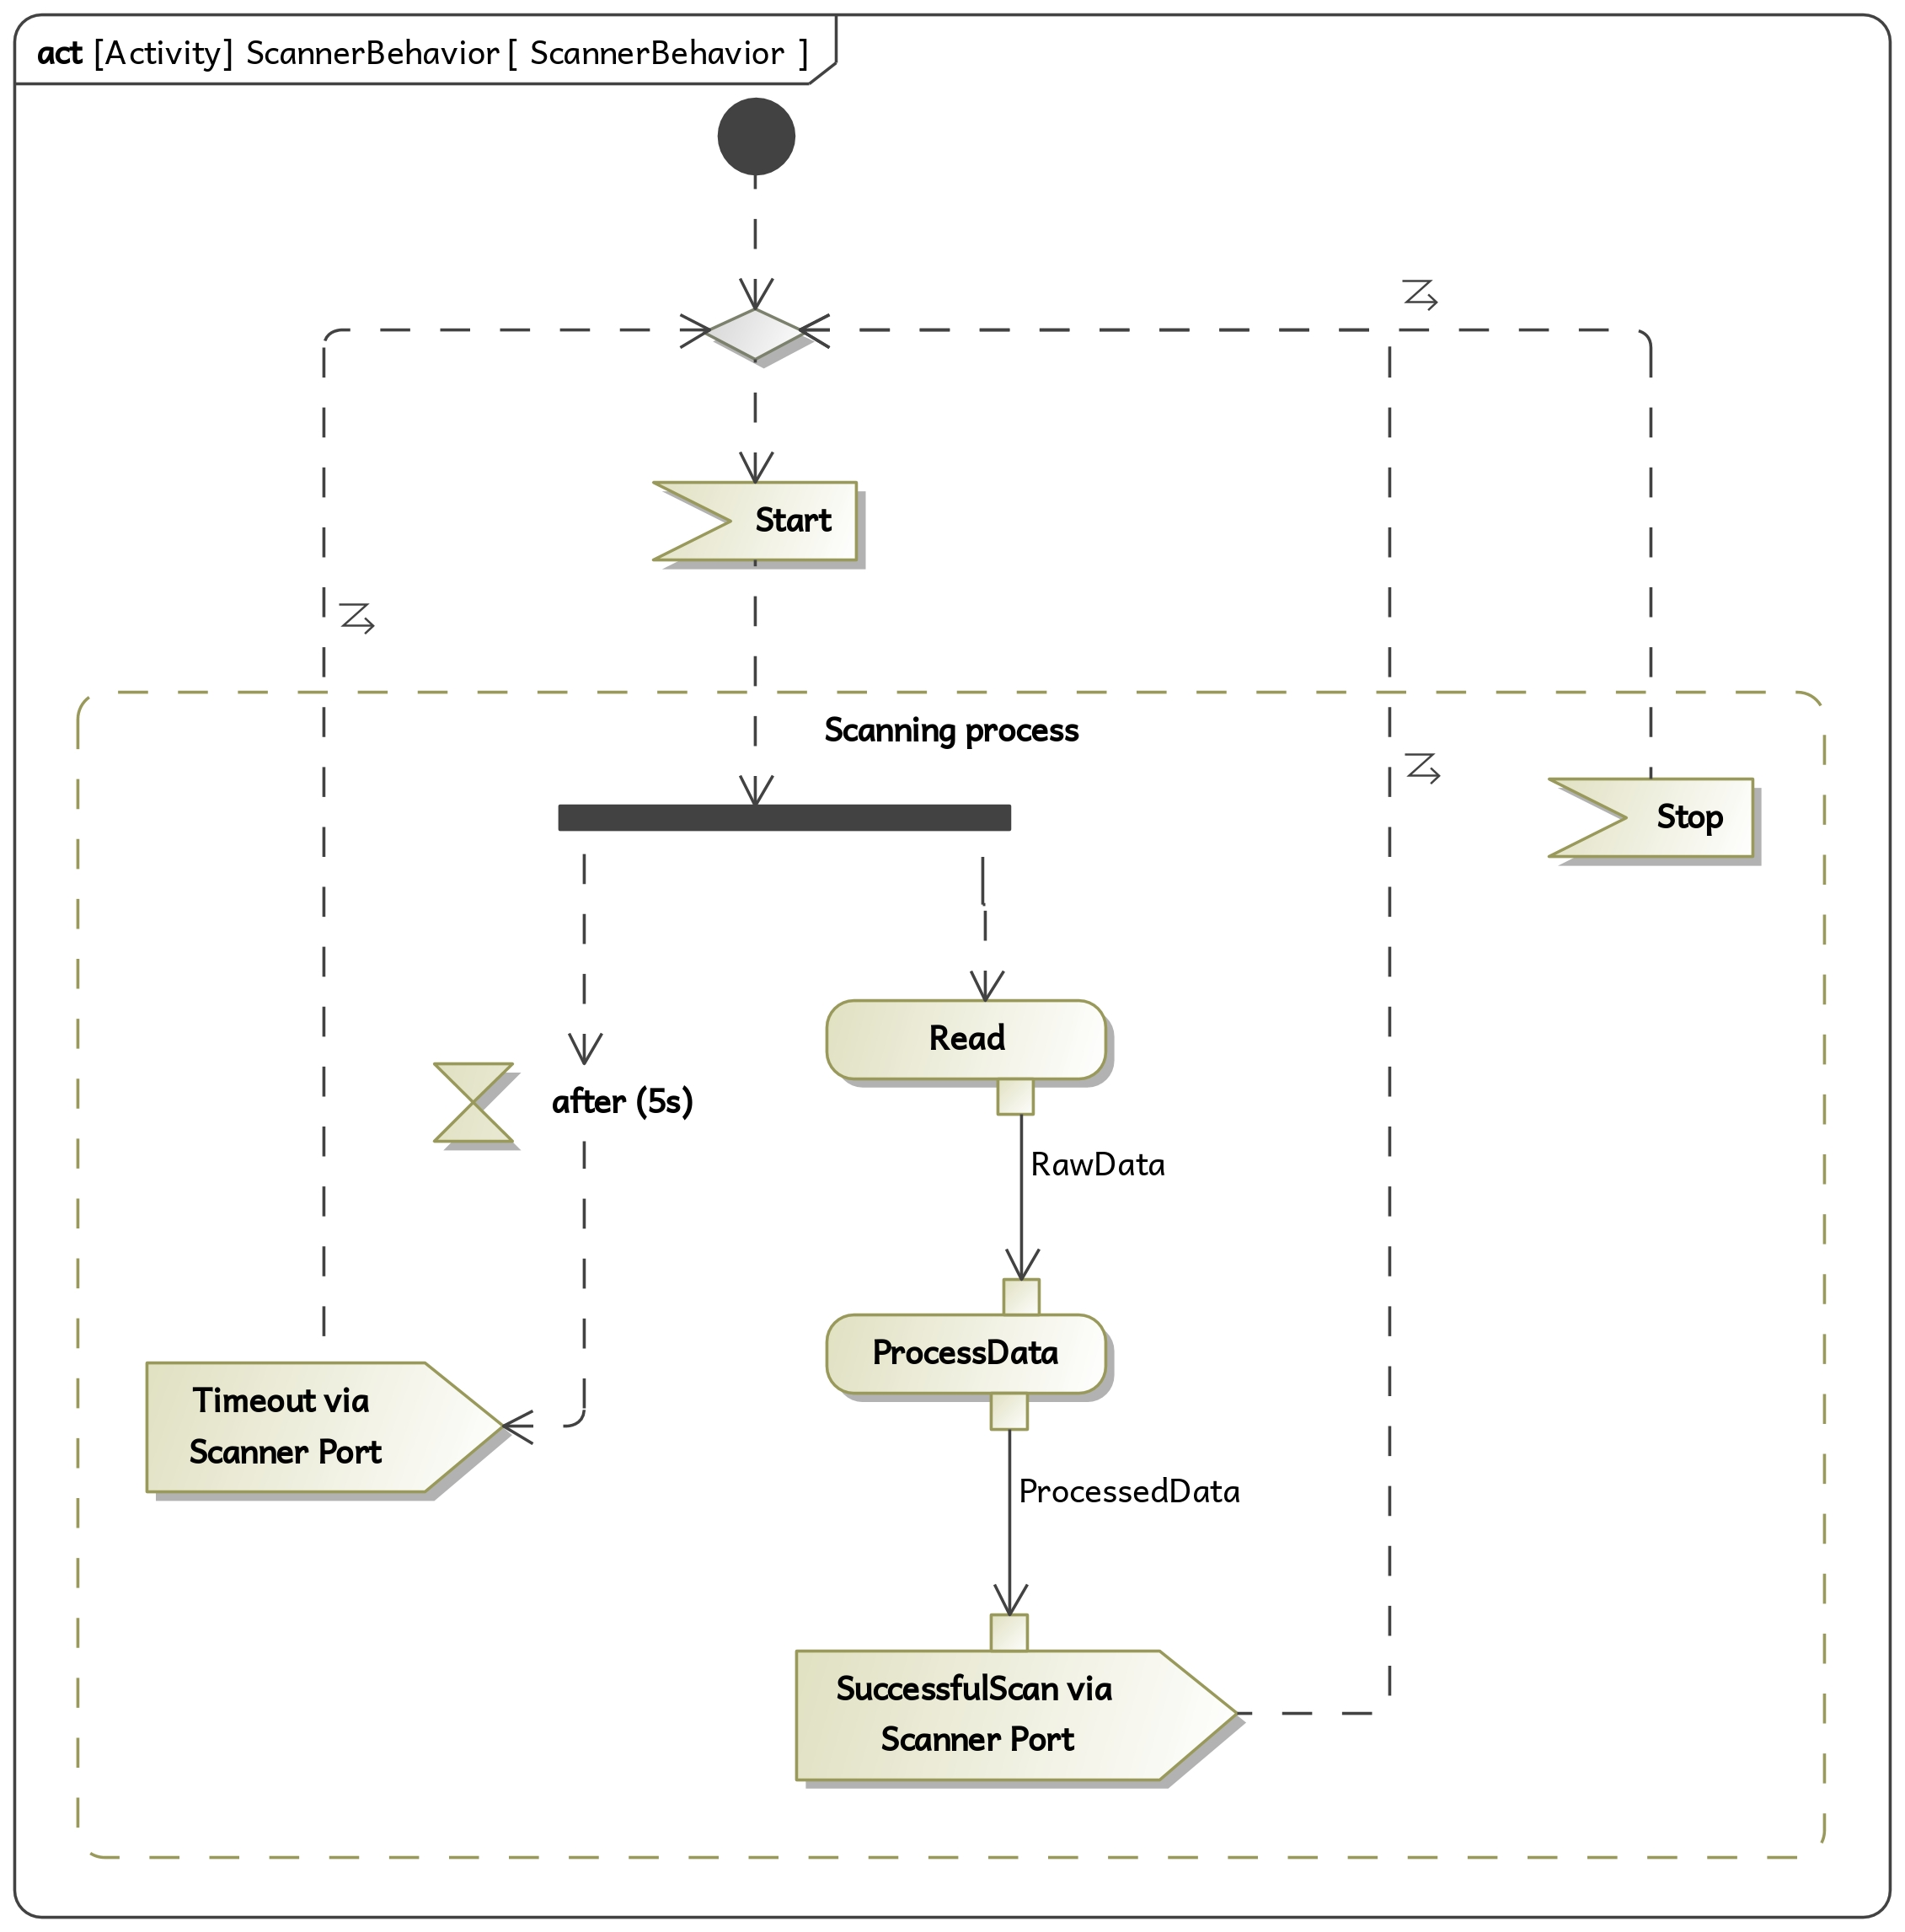
\includegraphics[width=\textwidth]{act-ScannerBehavior.jpg}
	\caption{Activity diagram of the \gls{RFIDScanner}'s behaviour}%
	\label{fig:act-ScannerBehavior}
\end{figure}


% - - - - - - - - - - - - - - - - - - - - - - - - - - - - - - - - - - - - - - -
\subsection{Boarding contoller behaviour}

The \gls{boardingController} is the most complex component of the boarding
equipment. Whereas the controlled components (\gls{turnstile},
\gls{RFIDScanner}, door, and alarm) are relatively simple, this controller unit
can be considered slightly intelligent. For example, when the door is blocked
and cannot close, it simply sends a \texttt{Blocked} signal to the controller
and stays opened. The component responsible for actually trying to close the
door again is the \gls{boardingController}.

\cref{fig:stm-ControllerBehavior} shows the state machine representation of the
controller's behaviour. All the actions seen on the transitions are defined as
activity digrams on \cref{fig:stm-ControllerBehavior-actions}.

Initially, the controller does nothing and waits for the bus to stop and to
receive the \texttt{StartBoarding} signal. When this happens, the boarding phase
begins and an \texttt{Open} signal is sent to the door. The door responds with
\texttt{Opened} signal when successfully opened. Then, the passenger is
autorhized by means of the \gls{RFIDScanner}. In the event of the person being
unathorized, the \gls{alarm} is turned on for five hundred milliseconds and the
next—or potentially the same—RFID is scanned. Otherwise, if the person is
allowed to board, the \gls{turnstile} is unlocked (by sending an \texttt{Unlock}
signal) and the passenger has five seconds to get on the bus. After the
\gls{turnstile} is rotated or the five second window expires, it is locked again
and the contoller instructs the \gls{RFIDScanner} to start (ie read). In case
the \gls{turnstile} cannot lock (this can happen when the \texttt{Lock} signal
is received during rotating), it sends a \texttt{Fail} signal and the
\gls{boardingController} attempts to lock it again every second until
successful. The \gls{turnstile} communicates succesful locking by sending an
\texttt{OK} signal.

When the controller receives the \texttt{FinishBoarding} signal, it is to stop
all boarding-related activities within ten seconds and send on \texttt{OK}
signal. This includes locking the \gls{turnstile} and closing the door. Both of
these must be successful (indicated by an \texttt{OK} signal from the
\gls{turnstile} and a \texttt{Closed} signal from the door) for the controller
to commence sending the \texttt{OK} signal and return to waiting for the
\texttt{StartBoarding} signal. Additionally, the \gls{RFIDScanner}'s operation
is aborted (by means of the \texttt{Stop} signal) and the \gls{alarm} is turned
on for the duration of the finishing phase. Just before sending the \texttt{OK}
signal, the alarm is turned off. In case these operations fail to complete
within the allocated ten seconds, the controller turns off the alarm, sends an
\texttt{Error} signal and shuts down.

\textbf{As per the critical requirements, the door must not be opened before the
	\texttt{StartBoarding} signal is received. We assumed that nothing
	interferes with the operation of the doors (by for example sending an
	\texttt{Open} signal to them) except the \gls{boardingController}.
	Therefore the doors are in their initial \texttt{Closed} state when the
	controller starts its operation. According to the diagram, the door must
	be closed within ten seconds after receiving the \texttt{FinishBoarding}
	signal, otherwise the whole component shuts down as a result of this
	failure. Otherwise the doors are certainly closed before continuing to
	listen to the \texttt{StartBoarding} signal.}

\begin{figure}
	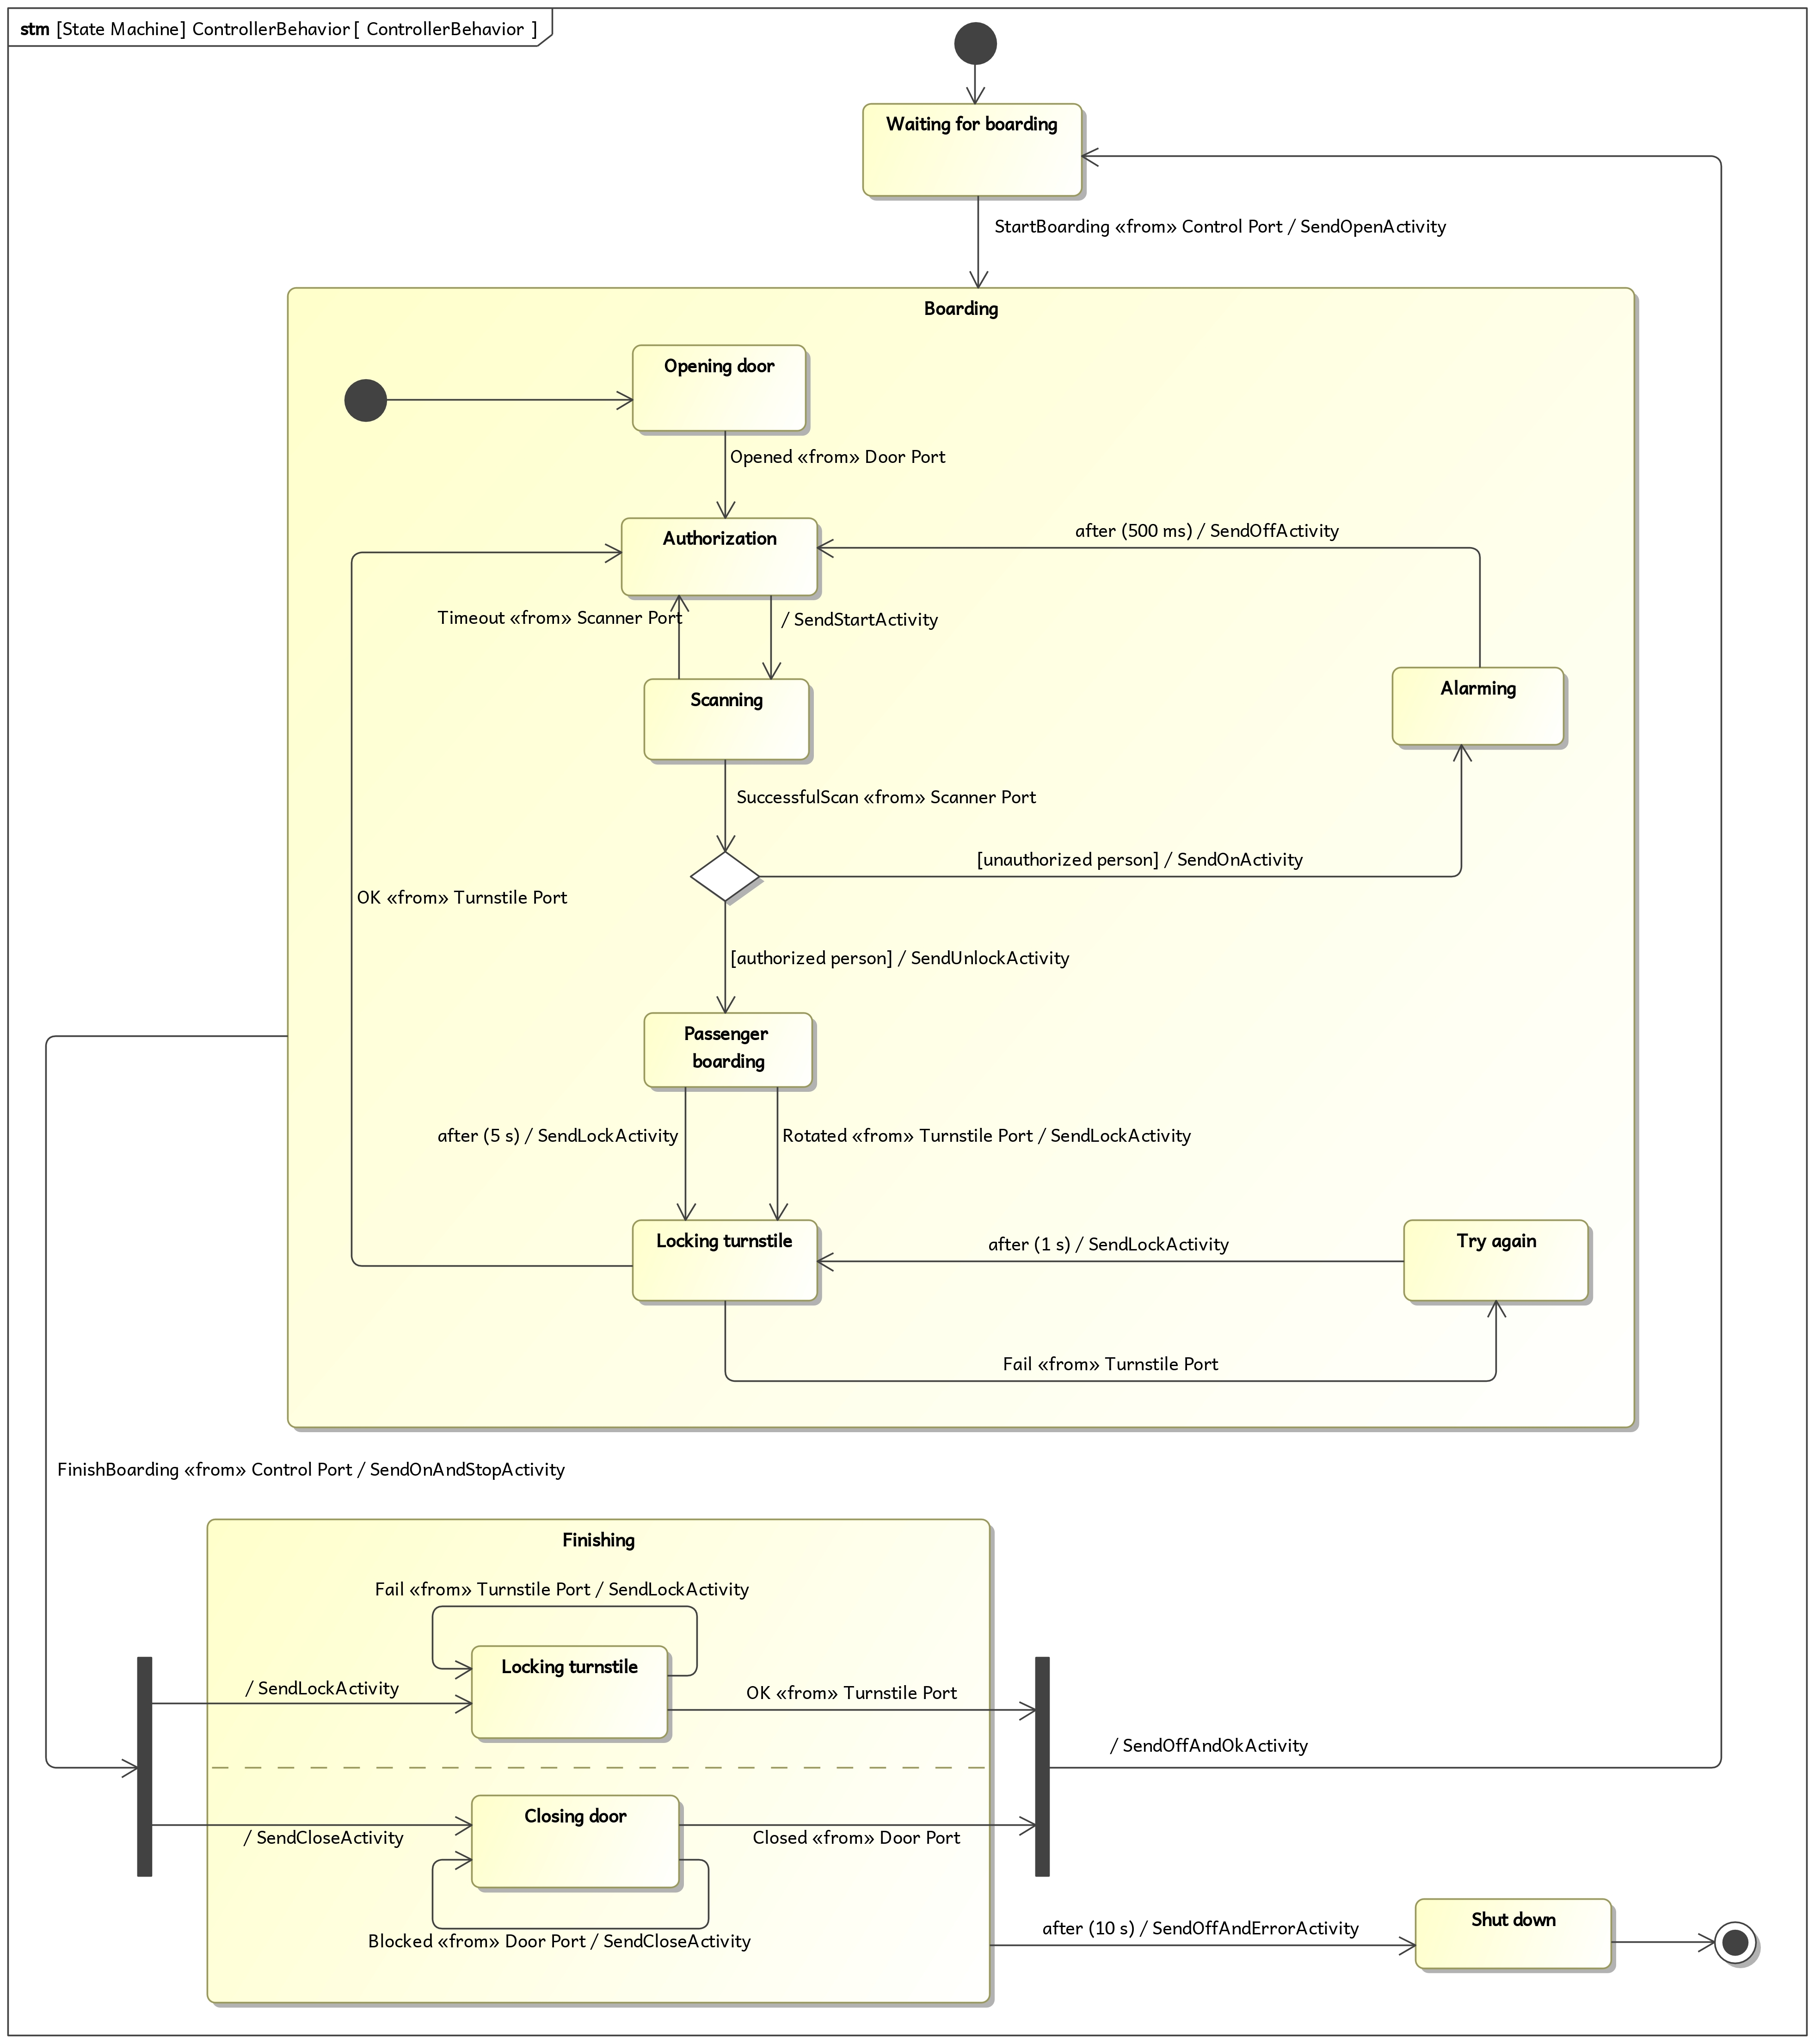
\includegraphics[width=\textwidth]{stm-ControllerBehavior.jpg}
	\caption{The state machine representation of the
		\gls{boardingController}'s behaviour}%
	\label{fig:stm-ControllerBehavior}
\end{figure}

\begin{figure}
	\begin{subfigure}{.33\textwidth}
		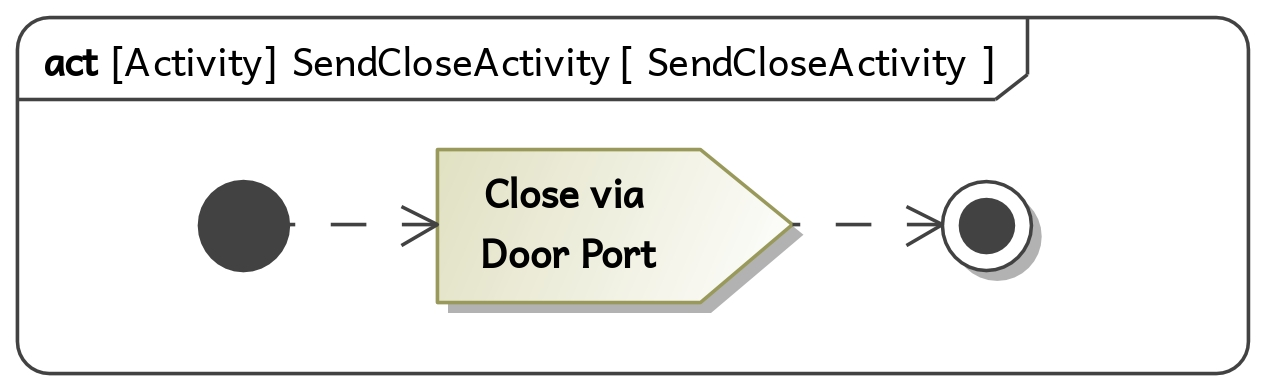
\includegraphics[width=\textwidth]
		{stm-ControllerBehavior-SendCloseActivity.jpg}
	\end{subfigure}
	\begin{subfigure}{.33\textwidth}
		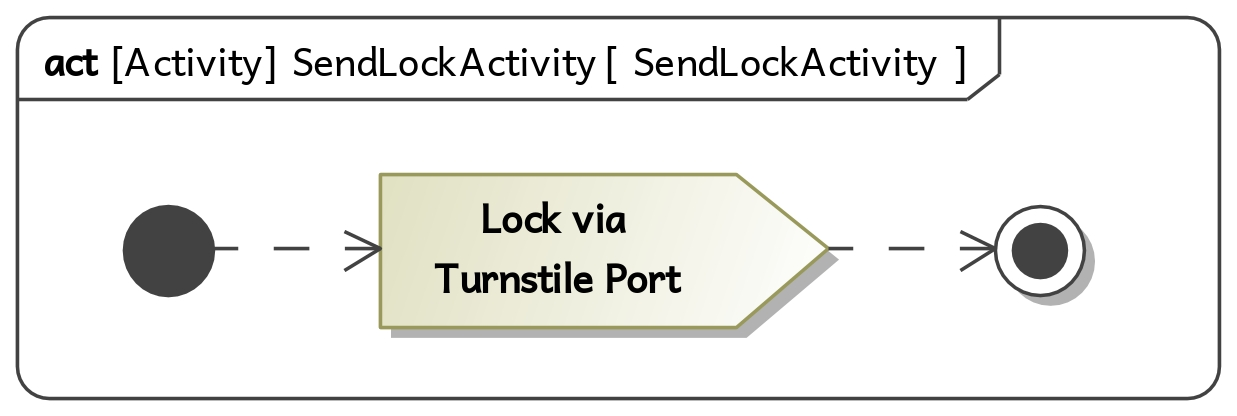
\includegraphics[width=\textwidth]
		{stm-ControllerBehavior-SendLockActivity.jpg}
	\end{subfigure}
	\begin{subfigure}{.33\textwidth}
		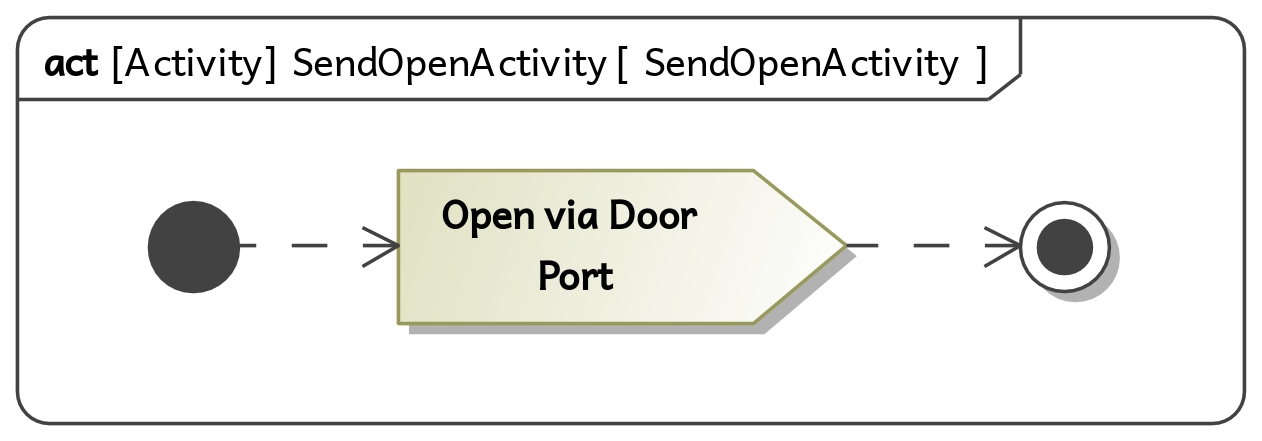
\includegraphics[width=\textwidth]
		{stm-ControllerBehavior-SendOpenActivity.jpg}
	\end{subfigure}
	% below
	\begin{subfigure}{.33\textwidth}
		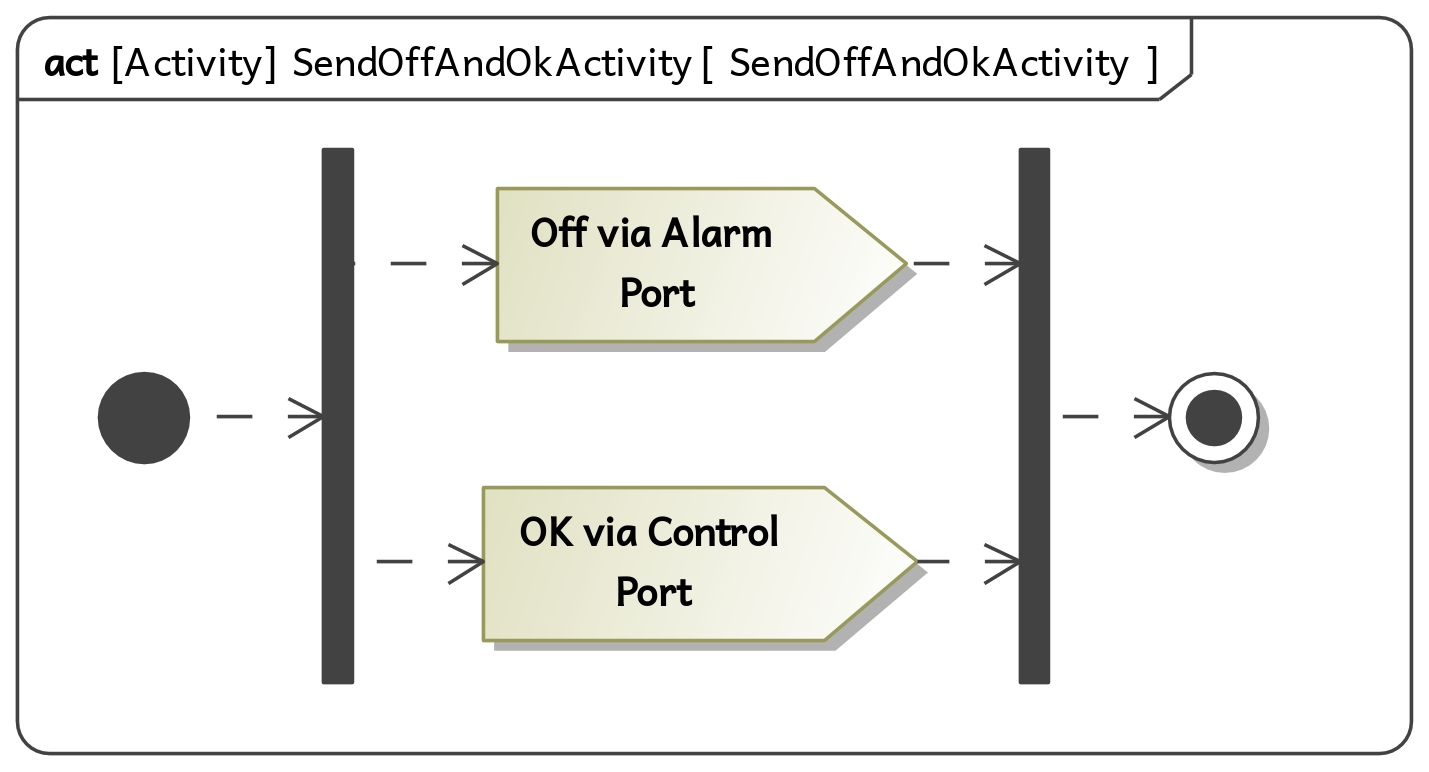
\includegraphics[width=\textwidth]
		{stm-ControllerBehavior-SendOffAndOkActivity.jpg}
	\end{subfigure}
	\begin{subfigure}{.33\textwidth}
		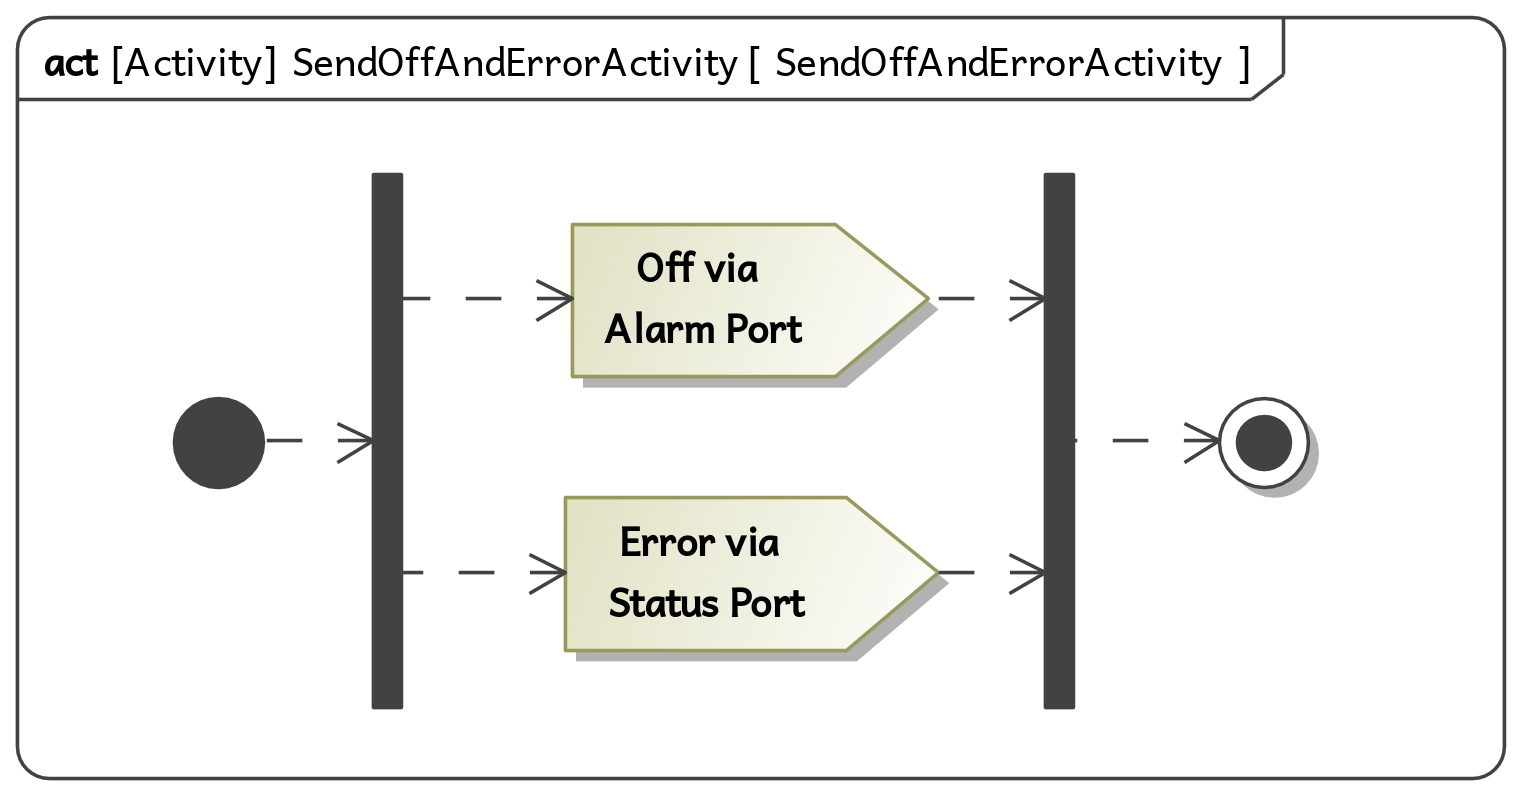
\includegraphics[width=\textwidth]
		{stm-ControllerBehavior-SendOffAndErrorActivity.jpg}
	\end{subfigure}
	\begin{subfigure}{.33\textwidth}
		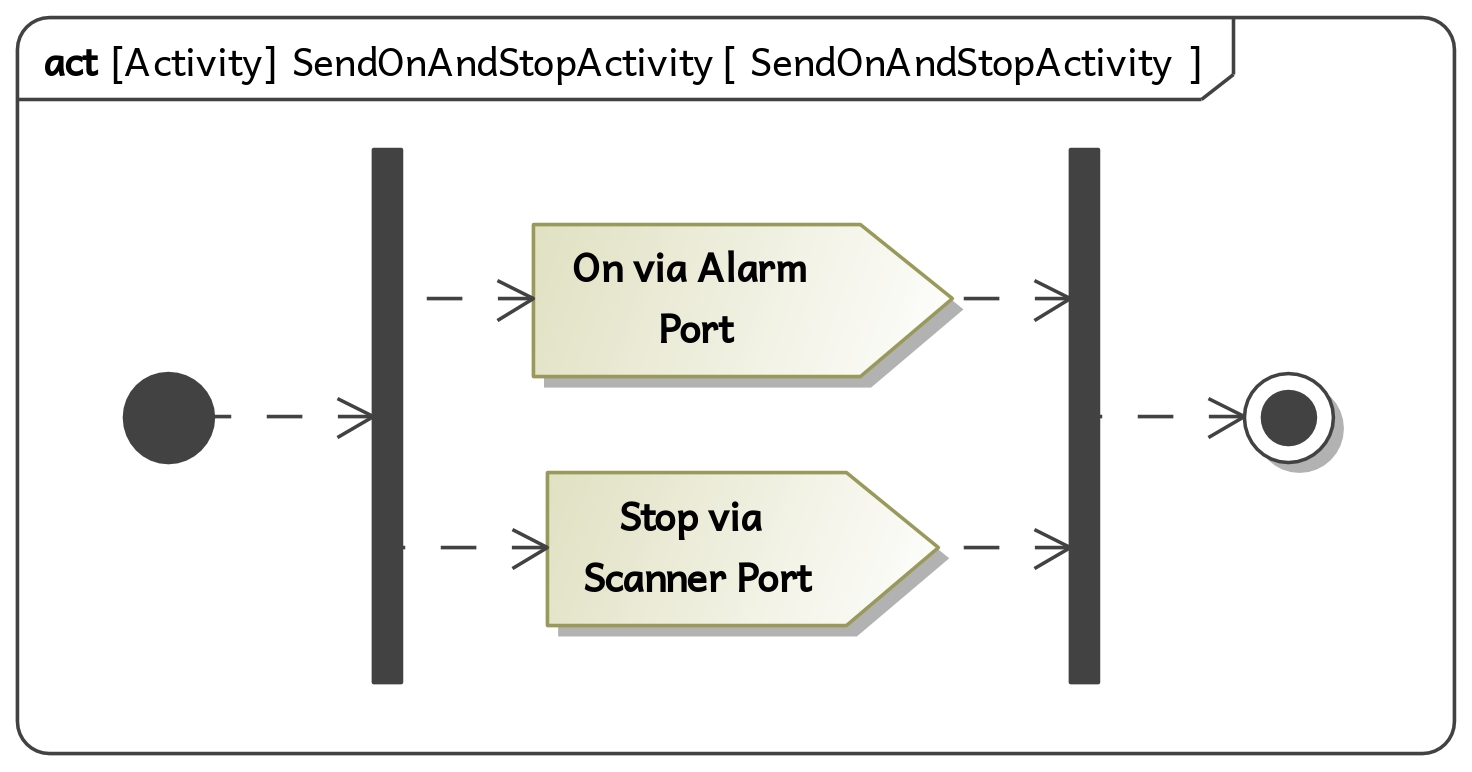
\includegraphics[width=\textwidth]
		{stm-ControllerBehavior-SendOnAndStopActivity.jpg}
	\end{subfigure}
	\caption{Activity diagrams for the actions seen on transitons on
		\cref{fig:stm-ControllerBehavior}}%
	\label{fig:stm-ControllerBehavior-actions}
\end{figure}

% ------------------------------------------------------------------------------
\section{Work journal}

\begin{tabularx}{\textwidth}{l l l X}
	\toprule
	Team member & Date & Time\footnote{in hours} & Activity \\ \midrule

	% TODO
	\bottomrule
\end{tabularx}

\clearpage
\glsaddall
\printglossaries

\end{document}
